\documentclass[11pt]{article}
\usepackage{amssymb,amsmath,amsthm,url,graphicx}
\usepackage {listings}
\usepackage{fancyhdr}

\def\shownotes{1}   % set 1 for version with author notes
                    % set 0 for no notes



%uncomment to get hyperlinks
%\usepackage{hyperref}

%%%%%%%%%%%%%%%%%%%%%%%%%%%%%%%%%%%%%%%%%%%%%%%%%%%%%%%%%%%%%%
%Some macros (you can ignore everything until "end of macros")

\topmargin 0pt \advance \topmargin by -\headheight \advance
\topmargin by -\headsep

\textheight 8.9in

\oddsidemargin 0pt \evensidemargin \oddsidemargin \marginparwidth
0.5in

\textwidth 6.5in

%%%%%%

\providecommand{\vs}{vs. }
\providecommand{\ie}{\emph{i.e.,} }
\providecommand{\eg}{\emph{e.g.,} }
\providecommand{\cf}{\emph{cf.,} }
\providecommand{\etc}{\emph{etc.} }

\newcommand{\getsr}{\gets_{\mbox{\tiny R}}}
\newcommand{\bits}{\{0,1\}}
\newcommand{\bit}{\{0,1\}}
\newcommand{\Ex}{\mathbb{E}}
\newcommand{\eqdef}{\stackrel{def}{=}}
\newcommand{\To}{\rightarrow}
\newcommand{\e}{\epsilon}
\newcommand{\R}{\mathbb{R}}
\newcommand{\N}{\mathbb{N}}
\newcommand{\Gen}{\mathsf{Gen}}
\newcommand{\Enc}{\mathsf{Enc}}
\newcommand{\Dec}{\mathsf{Dec}}
\newcommand{\Sign}{\mathsf{Sign}}
\newcommand{\Ver}{\mathsf{Ver}}
\renewcommand\qedsymbol{$\blacksquare$}


\providecommand{\mypara}[1]{\smallskip\noindent\emph{#1} }
\providecommand{\myparab}[1]{\smallskip\noindent\textbf{#1} }
\providecommand{\myparasc}[1]{\smallskip\noindent\textsc{#1} }
\providecommand{\para}{\smallskip\noindent}

\usepackage{mathtools}
\usepackage{amsthm}
\DeclarePairedDelimiter\ceil{\lceil}{\rceil}
\DeclarePairedDelimiter\floor{\lfloor}{\rfloor}

\theoremstyle{definition}
\newtheorem{ex}{Exercise}
\newtheorem{definition}{Definition}
\newtheorem{theorem}{Theorem}[section]
\newtheorem{corollary}{Corollary}[theorem]
\newtheorem{lemma}[theorem]{Lemma}

%%%%%%%  Author Notes %%%%%%%
%
\ifnum\shownotes=1
\newcommand{\authnote}[2]{{ $\ll$\textsf{\footnotesize #1 notes: #2}$\gg$}}
\else
\newcommand{\authnote}[2]{}
\fi
\newcommand{\Snote}[1]{{\authnote{Solution}{#1}}}
\newcommand{\Inote}[1]{{\authnote{Solution}{#1}}}
\newcommand{\Ichanged}[1]{{\authnote{Changed}{#1}}}
%%%%%%%%%%%%%%%%%%%%%%%%%%%%%%%%%

\newcommand{\VAR}{\mathrm{VAR}}



% end of macros
%%%%%%%%%%%%%%%%%%%%%%%%%%%%%%%%%%%%%%%%%%%%%%%%%%%%%%%%%%%%%%


% page counting, header/footer
\usepackage{fancyhdr}
\usepackage{lastpage}
\usepackage{graphicx}
\usepackage[]{algorithm2e}

\pagestyle{fancy}
\lhead{\footnotesize \parbox{11cm}{LaTeX Workshop, Spring 2018} }
\rhead{Your Name}
\renewcommand{\headheight}{24pt}

\begin{document}

\title{Your Title}
\author{Author Name}
\maketitle

\myparab{Collaborators: } Katie Quirk, Armin Sabouri \\

\noindent\hrulefill


\thispagestyle{fancy}
 
\begin{enumerate}
\item[A.] Basic text styling: \\
\\
\underline{This will underline your text.} \\
\\
\textit{This will italicize your text.}\\
\\
\textbf{This will bold your text.}

\item[B.] Pictures and Images %change for what you want your item to be
    \begin{enumerate}
    \item[1.] Picture of a Giraffe: \\
    \\
    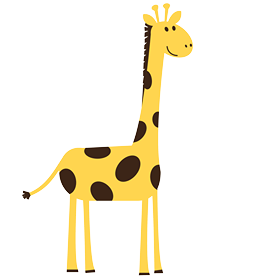
\includegraphics[scale=0.2]{giraffe-clipart-1.png}    %include pictures
        % scale picture to fit
    \\
    \item[2.] 
    \\
    \end{enumerate}
    
\item [C.] Math mode
    \begin{enumerate}
        \item[i.] When you want to enter mathematical symbols, they must be wrapped by \$.
        \\
        \item[ii.] 
            \begin{enumerate}
            \item $\frac{1}{m-1} \sum_{a,b}^{} v_{a}v_{b} $
            \item $\frac{1}{m-1} \sum_{a} v_{a} \sum_{b}v_{b} $
            \item $\frac{1}{m-1} \sum_i(\sum_{a} v_{a} \sum_{b}v_{b}) $
            \item $\frac{1}{m-1} (\sum_{i \in m}\sum_{a} v_{a}) (\sum_{i \in m}\sum_{b}v_{b}) $
            \item $\frac{1}{m-1} (\sum_{i \in m}c_i) (\sum_{i \in m}c_i) $
            \item $\frac{1}{m-1} (\sum_{i \in m}c_i)^{2} $
            \end{enumerate}
            Thus, $\frac{1}{m-1} (\sum_{i \in m}c_i)^{2} $ = $\frac{1}{m-1} \sum_{a,b}^{} v_{a}v_{b} $.
        \\
        \\
        \item[iii.] You may want specific spacing in math mode: \\
        \\
            $
            S = \{ z \in \mathbb{C}\, |\, |z| < 1 \} \quad \textrm{and} \quad S_2=\partial{S}
            $
            \\
        \item[iv.] $\lceil x / 2 \rceil$
        \\
        \item[v.] matrices: \\
        \\
        $
            A=
            \begin{bmatrix}
            1 & 3 \\
            2 & 2 \\
            3 & 3
            \end{bmatrix}
            \\
            B=
            \begin{bmatrix}
            2 & 2 & 4 \\
            1 & 2 & 3
            \end{bmatrix}
            
         $
    \end{enumerate}
    
\item [D.] Pseudocode/Code: \\

\begin{lstlisting} [language = python]
for i in range(3,9):
    print ("Hello ", i)
    
\end{lstlisting}
\\

\item[E.] Proofs/Theorems: \\
\begin{theorem}
Let $f$ be a function whose derivative exists in every point, then $f$ is 
a continuous function.
\end{theorem}
 
\begin{theorem}[Pythagorean theorem]
\label{pythagorean}
This is a theorema about right triangles and can be summarised in the next 
equation 
\[ x^2 + y^2 = z^2 \]
\end{theorem}
 
And a consequence of theorem \ref{pythagorean} is the statement in the next 
corollary.
 
\begin{corollary}
There's no right rectangle whose sides measure 3cm, 4cm, and 6cm.
\end{corollary}
 
You can reference theorems such as \ref{pythagorean} when a label is assigned.
 
\begin{lemma}
Given two line segments whose lengths are $a$ and $b$ respectively there is a 
real number $r$ such that $b=ra$.
\end{lemma}

\begin{proof}
To prove it by contradiction try and assume that the statement is false,
proceed from there and at some point you will arrive to a contradiction.
\end{proof}

\end{enumerate}


\noindent\hrulefill % this creates a line across the page

\section*{New Section}

This can be an alternative way to break up your questions.

\end{document}
